% https://tikz.dev/tikz-arrows
% https://tikz.net/contents/chapter-03-drawing-positioning-and-aligning-nodes/

\usepackage{tikz}
\usetikzlibrary{positioning, tikzmark, calc, shapes.geometric, arrows}
% \usetikzlibrary{positioning,tikzmark,calc,arrows,shapes,backgrounds,fit}

\newenvironment{myTree}
{
    \begingroup
    \begin{center}
    \begin{tikzpicture}[level distance=1.5cm, level 1/.style={sibling distance=3cm}, level 2/.style={sibling distance=1.5cm}]
}
{
    \end{tikzpicture}
    \end{center}
    \endgroup
}


\newenvironment{myTreeLThree}
{
    \begingroup
    \begin{center}
    \begin{tikzpicture}[level distance=1.5cm, level 1/.style={sibling distance=6cm}, level 2/.style={sibling distance=3cm}, level 3/.style={sibling distance=1.5cm}]
}
{
    \end{tikzpicture}
    \end{center}
    \endgroup
}

\newenvironment{vArrow}[3][black]
{
    \draw[->, #1] (#2) -- (#3);
}
{

}

\newenvironment{tArcDown}[2][black]
{
    \draw[-latex,#1] ($#2$) arc [ start angle=-160, end angle=-20, x radius=0.9cm, y radius =0.7cm ] ;
}
{

}


\newenvironment{tArcUp}[2][red]
{
    \draw[-latex,#1] ($#2$) arc [ start angle=160, end angle=20, x radius=0.9cm, y radius =0.7cm ] ;
}
{

}

\tikzstyle{flowchart-start} = [rectangle, rounded corners,
minimum width=3cm,
minimum height=1cm,
text centered,
draw=black,
fill=red!30]

\tikzstyle{flowchart-io} = [trapezium,
trapezium stretches=true, % A later addition
trapezium left angle=70,
trapezium right angle=110,
minimum width=3cm,
minimum height=1cm, text centered,
draw=black, fill=blue!30]

\tikzstyle{flowchart-process} = [rectangle,
minimum width=3cm,
minimum height=1cm,
text centered,
text width=6cm,
draw=black,
fill=orange!30]

\tikzstyle{flowchart-decision} = [diamond,
minimum width=3cm,
minimum height=1cm,
text centered,
draw=black,
fill=green!30]

\tikzstyle{flowchart-arrow} = [thick,->,>=stealth]




\begin{comment}

    \begin{center} 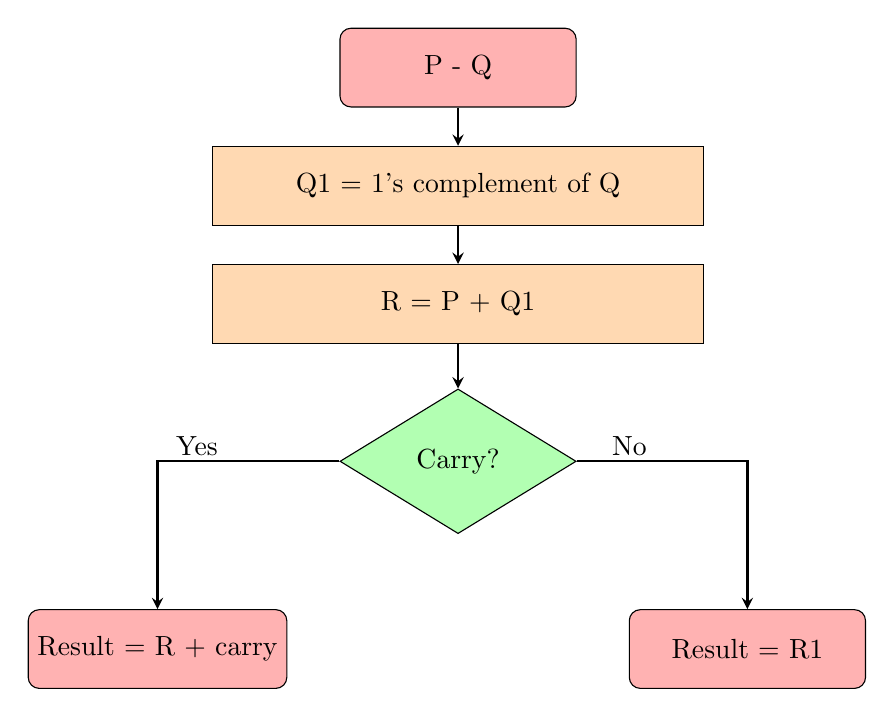
\begin{tikzpicture}[node distance=1.5cm]
        \node (start) [flowchart-start] {P - Q};
        \node (S1) [flowchart-process, below of=start] { Q1 = 1's complement of Q };
        \node (S2) [flowchart-process, below of=S1] { R = P + Q1 };
        \node (S3) [flowchart-decision, below of=S2, yshift=-0.5cm] { Carry? };xx
        \node (S4) [flowchart-start, below left=2cm of S3] { Result = R + carry};
        \node (S5) [flowchart-start, below right=2cm of S3] {Result = R1};

        \draw [flowchart-arrow] (start) -- (S1); \draw [flowchart-arrow] (S1) -- (S2); \draw [flowchart-arrow] (S2) -- (S3);
        \draw [flowchart-arrow] (S3.west) -| node[right of= S3, xshift=-1cm, yshift=0.2cm] {Yes} (S4.north);
        \draw [flowchart-arrow] (S3.east) -| node[right of= S3, xshift=-3cm, yshift=0.2cm] {No} (S5.north);

    \end{tikzpicture} \end{center}

\end{comment}
